%!TEX root = ../LA2.tex
\section{Quadratische Polynome und Quadriken}
\label{sec:2.8}

Wir wollen die Diagonalisierbarkeit von selbstadjungierten Matrizen ausnutzen, um in diesem Abschnitt quadratische Polynome auf $\RR^n$ zu untersuchen.

\begin{definition}[Quadratisches Polynom]
	\label{def:8.1}
	Eine Abbildung $p \colon \RR^n \rightarrow \RR$ heißt \Index{quadratisches Polynom}, wenn $b_{ij}, \alpha_j, \alpha \in \RR, 1 \leq i,j \leq n$ existieren, sodass für alle $x = (x_1,\dots,x_n)^T \in \RR^n$ gilt:
	\[
		p((x_1,\dots,x_n)^T) = \sum_{i,j=1}^{n} b_{ij} x_i x_j + \sum_{j=1}^{n} \alpha_j x_j + \alpha.
	\]
\end{definition}

Die $x_ix_j = x_jx_i$, können wir in der Formel die $b_{ij}$ durch $a_{ij} := \frac{1}{2}(b_{ij} + b_{ji})$ ersetzen, und erhalten dann $a_{ij} = a_{ji}$.
Ist dann $A = (a_{ij})_{ij} \in M(n \times n, \RR)$, so ist $A = A^T$ und wir erhalten
\[
	p((x_1,\dots,x_n)^T) = \sum_{i,j=1}^{n} a_{ij} x_i x_j + \sum_{j=1}^{n} \alpha_j x_j + \alpha.
\]

\begin{lemma}
	\label{lemma:8.2}
	Ist $A = A^T$ wie oben und ist $a := \frac{1}{2} \cdot (\alpha_1,\dots,\alpha_n) \in \RR^n$, so gilt für alle $x \in \RR^n$:
	\[
		p(x) = \sk{Ax,x} + 2 \sk{a,x} + \alpha = x^T A x + 2 a^T x + \alpha.
	\]
\end{lemma}

\begin{beweis}
	Die erste Gleichung folgt direkt durch einsetzen.
	Die zweite Gleichung folgt aus $\sk{y,x} = y^Tx$ für alle $x,y \in \RR^n$ und $\sk{Ax,x} = \sk{x,A^Tx} = \sk{x,Ax} = x^T Ax$. \qedhere
\end{beweis}

Unser Ziel: Wir wollen durch geeignete Wahl von Koordinaten in $\RR^n$ und durch Verschiebung des Ursprungs erreichen, dass $p$ eine besonders schöne Gestalt annimmt (vgl. mit Blatt 6, Aufgabe 1).
Beachte: Der Faktor $2$ vor dem Term $\sk{a,x}$ bzw. $a^Tx$ vereinfacht einige Umformungen!

\begin{lemma}
	\label{lemma:8.3}
	Sei $A \in M(n \times n,\RR)$ mit $A = A^T$.
	Dann gilt $\Bild(A) = \Bild(A^2)$.
	Insbesondere existiert zu jedem $a \in \RR^n$ ein $c \in \RR^n$ mit $A^2c = -Aa$.
\end{lemma}

\begin{beweis}
	Sei $\{v_1,\dots,v_n\}$ eine Orthonormalbasis aus Eigenvektoren von $A$ mit zugehörigen Eigenwerten $\lambda_1,\dots,\lambda_n$.
	Die Reihenfolge der Eigenvektoren und Eigenwerte sei so gewählt, dass $\lambda_1,\dots,\lambda_k \neq 0$ und (falls $k \leq n$) $\lambda_{k+1}, \dots, \lambda_n = 0$.
	Dann folgt für ein $v = \sum_{i=1}^{n} \mu_i v_i$:
	\[
		Av = \sum_{i=1}^{n} \mu_i Av_i = \sum_{i=1}^{n} \mu_i \lambda_i v_i = \sum_{i=1}^{k} \mu_i \lambda_i v_i.
	\]
	Setzen wir dann $w := \sum_{i=1}^{k} \frac{\mu_i}{\lambda_i} v_i$, so folgt
	\[
		A^2w = A \cdot \enb{\sum_{k=1}^{n} \frac{\mu_i}{\lambda_i} Av_i} = A \cdot \enb{\sum_{i=1}^{k} \mu_i v_i} = \sum_{i=1}^{n} \mu_i \lambda_i v_i = Av.
	\]
	Damit folgt $\Bild(A) \subseteq \Bild(A^2)$.
	Die Umkehrung ist trivial. \qedhere
\end{beweis}

\begin{lemma}[Reduktion durch Translation]
	\label{lemma:8.4}
	Sei $p(x) = x^T A x + 2a^Tx + \alpha$ mit $A = A^T \in M(n \times n, \RR), a \in \RR^n$ und $\alpha \in \RR$.
	Ferner sei $c \in \RR^n$ mit $A^2c = -Aa$ (existiert nach \autoref{lemma:8.3}) und sei $b := Ac + a$.
	Dann gelten:
	\begin{enumerate}[(i)]
		\item $p(x+c) = x^T Ax + 2b^Tx + p(c)$ und $Ab = 0$.
		\item Ist $b = 0$, so folgt $p(x+c) = x^TAx + p(c)$ (kein linearer Term).
		\item Ist $b \neq 0$, so gilt für $d := c+\delta b$ mit $\delta := - \frac{p(c)}{2 \no{b}^2}$: $p(x+d) = x^TAx + 2b^Tx$ (kein konstanter Term).
	\end{enumerate}
\end{lemma}

\begin{beweis}
	Zunächst gilt für alle $x,y\in \RR^n$:
	\begin{align*}
		p(x+y) &\stack{}{=} (x+y)^T A (x+y) = 2a^T(x+y) + \alpha \\
		&\stack{}{=} x^T Ax + 2y^T Ax + y^T Ay + 2a^Tx + 2a^Ty + \alpha \\
		&\stack{A=A^T}{=} x^TAx + 2(Ay + a)^Tx + p(y).
	\end{align*}
	\begin{enumerate}[(i)]
		\item Die Gleichung $p(x+c) = x^TAx + 2b^Tx + p(c)$ folgt auch obiger Rechnung mit $b = Ac+a$.
		Da $A^2c = -Aa$, folgt $Ab = A(Ac + a) = A^2c + Aa = 0$.
		\item folgt sofort aus (i).
		\item Sei $d = c + \delta b$ wie in (iii).
		Dann gilt
		\begin{align*}
			p(x+d)& \stack{}{=} x^TAx + 2(Ad+a)^T x + p(d) \\
			&\stack{}{=} x^TAx + 2(A(c+\delta b) + a)^T x + p(d) \\
			&\stack{Ab=0}{=} x^TAx + 2\Underbrace{(Ac+a)}{=b}^Tx + p(d) = x^TAx + 2b^Tx + p(d).
		\end{align*}
	\end{enumerate}
	Zeige nun $p(d) = 0$.
	Es gilt
	\begin{align*}
		p(d) &= p(c+\delta b) = c^TAc + 2(\overbrace{A\delta b}^{\mathclap{=0}}+a)^T c + p(\delta b) \\
		&= p(c) - \alpha + p(\delta b) = p(c) - \alpha + \delta^2 b^TAb + \delta 2 a^T b + \alpha \\
		&= p(c) - p(c) \enb{\frac{1}{2 \no{b}^2}} 2a^Tb = 0,
	\end{align*}
	denn $\no{b}^2 = b^Tb = (Ac+a)^Tb = c^T\Underbrace{Ab}{=0} + a^Tb = a^Tb$. \qedhere
\end{beweis}

\begin{satz}[Normalform quadratischer Polynome I]
	\label{satz:8.5}
	Sei $p(x) = x^TAx + 2a^Tx + \alpha$ ein quadratisches Polynom auf $\RR^n$ mit $A = A^T$.
	Dann gilt:
	\begin{enumerate}[(i)]
		\item Ist $a \in \Bild(A)$, so existiert ein $O \in \oh(n)$, ein $d \in \RR^n$ und $\lambda_1,\dots,\lambda_n,\beta \in \RR$ mit
		\[
			p(Ox + d) = \lambda_1 x_1^2 + \dots + \lambda_n x_n^2 + \beta.
		\]
		\item Ist $a \notin \Bild(A)$, so existiert ein $O \in \oh(n), d \in \RR^n$ und $\lambda_1,\dots,\lambda_{n-1},\beta \in \RR$ mit
		\[
			p(Ox+d) = \lambda_1 x_1^2 + \dots + \lambda_{n-1} x_{n-1}^2 + \beta x_n.
		\]
	\end{enumerate}
\end{satz}

\begin{beweis}
	\mbox{} \\[-.9cm]
	\begin{enumerate}[(i)]
		\item Da $a \in \Bild(A)$, existiert ein $d \in \RR^n$ mit $Ad = -a$.
		Dann folgt $p(x+d) = x^TAx + 2(Ad+a)^Tx + p(d) = x^T Ax + p(d)$.
		Setze $B := p(d)$.
		Da $A = A^T$, existiert eine orthogonale Matrix $O \in \oh(n)$ mit $O^TAO = \diag(\lambda_1,\dots,\lambda_n)$.
		Dann folgt
		\begin{align*}
			p(Ox+d) &= (Ox)^TA(Ox) + \beta = x^T(O^TAO)x + \beta \\
			&= x^T(\diag(\lambda_1,\dots,\lambda_n))x + \beta = \lambda_1 x_1^2 + \dots + \lambda_n x_n^2 + \beta.
		\end{align*}
		\item Sei $c \in \RR^n$ mit $A^2c = -Aa$.
		Da $a \notin \Bild(A)$, ist dann $b := Ac + a \neq 0$.
		Nach \autoref{lemma:8.4}(iii) gilt dann für $d := c + \delta b$ mit $\delta = - \frac{p(c)}{2 \no{b}^2}$, dass $p(x+d) = x^TAx + 2b^Tx$.
		
		Wähle (mit Hilfe des Schmidtschen Orthonormalisierungsverfahrens) eine Orthonormalbasis $\{v_1,\dots,v_n\}$ von $\RR^n$ mit $v_n = \no{b}^{-1} \cdot b$.
		Ist dann $B := (v_1,\dots,v_n) \in \oh(n)$, so folgt
		\[
			b^TB = (b^Tv_1,\dots,b^Tv_n) = \no{b} (v_n^Tv_1,\dots,v_n^Tv_n) = (0,\dots,0,\no{b}).
		\]
		Dann folgt
		\begin{align*}
			p(Bx+d) &= (Bx)^T A (Bx) + 2b^T(Bx) \\
			&= x^T(B^TAB)x + 2(0,\dots,0,\no{b})^Tx \\
			&= x^T(B^TAB)x + 2 \no{b} x_n.
		\end{align*}
		Ferner gilt wegen $Ab = 0$, dass $Av_n = 0$, also $AB = (Av_1,\dots,Av_n) = (Av_1,\dots,Av_{n-1},0)$, und dann auch $B^TAB = (B^TAv_1, \dots, B^TAv_n,0)$.
		Wegen $(B^TAB)^T = B^TA^TB = B^TAB$, da $A^T = A$, ist $B^TAB$ symmetrisch, sodass die $n$-te Spalte und Zeile von $B^TAB$ null sind, also
		\[
			B^TAB = \enb{\begin{BMAT}[.25cm]{c|c}{c|c}
				\wt{A} & 0 \\
				0 & 0
				\end{BMAT}} \quad \text{mit } \wt{A}^T = \wt{A} \in M((n-1) \times (n-1),\RR).
		\]
		\newpage
		Nach \autoref{kor:7.16} existiert dann ein $S \in \oh(n-1)$ mit $S^T\wt{A}S = \diag(\lambda_1,\dots,\lambda_{n-1})$ für geeignete $\lambda_1,\dots,\lambda_{n-1} \in \RR$.
		Ist dann
		\[
		= B \cdot \enb{\begin{BMAT}[.25cm]{c|c}{c|c}
			S & 0 \\
			0 & 1
			\end{BMAT}},
		\]
		so ist $O \in \oh(n)$ mit
		\begin{align*}
			p(Ox+d) &= x^T(O^TAO)x + 2 \no{b} x_n \\
			&= x^T \cdot \enb{\begin{BMAT}[.25cm]{c|c}{c|c}
				S^T & 0 \\
				0 & 1
				\end{BMAT}} \cdot B^TAB \cdot \enb{\begin{BMAT}[.25cm]{c|c}{c|c}
				S & 0 \\
				0 & 1
				\end{BMAT}} \cdot x + 2 \no{b} x_n \\
			&= x^T \cdot \enb{\begin{BMAT}[.25cm]{c|c}{c|c}
				S^T\wt{A}S & 0 \\
				0 & 0
				\end{BMAT}} \cdot x + 2 \no{b} x_n \\
			&= x^T \cdot \diag(\lambda_1,\dots,\lambda_{n-1},0) \cdot x_n + 2 \no{b} x_n \\
			&= \lambda_1 x_1^2 + \dots + \lambda_{n-1}x_{n-1}^2 + \beta x_n
		\end{align*}
		für $\beta := 2 \no{b}$. \qedhere
	\end{enumerate}
\end{beweis}

Wenn wir die Koeffizienten $\lambda_i$ vor den quadratischen Termen in \autoref{satz:8.5} nach ihren Vorzeichen ordnen und $\lambda_i = \frac{1}{\rho_i^2}$, falls $\lambda_i > 0$, und $-\lambda_j = \frac{1}{\sigma_j^2}$, falls $\lambda_j < 0$, schreiben, so erhalten wir die folgenden Normalformen für quadratische Polynome auf $\RR^n$:

\begin{satz}[Normalformen quadratischer Polynome II]
	\label{satz:8.6}
	Sei $p(x) = x^TAx + 2a^Tx + \alpha$ ein quadratisches Polynom auf $\RR^n$ mit $A = A^T$.
	Dann gilt:
	\begin{enumerate}[(i)]
		\item Ist $a \in \Bild(A)$, so existiert ein $O \in \oh(n), d \in \RR^n, \rho_1, \dots, \rho_k, \sigma_{k+1},\dots,\sigma_{m}, \beta \in \RR$ mit $0 \leq k \leq m \leq n$ und
		\[
			p(Ox+d) = \frac{x_1^2}{\rho_1^2} + \dots \frac{x_k^2}{\rho_k^2} - \frac{x_{k+1}^2}{\sigma_{k+1}^2} - \dots - \frac{x_m^2}{\sigma_m^2} + \beta.
		\]
		\item Ist $a \notin \Bild(A)$, so existiert $O \in \oh(n), d \in \RR^n, \rho_1, \dots, \rho_k, \sigma_{k+1},\dots,\sigma_m,\beta \in \RR$ mit $0 \leq k \leq m \leq n-1$ und
		\[
		p(Ox+d) = \frac{x_1^2}{\rho_1^2} + \dots \frac{x_k^2}{\rho_k^2} - \frac{x_{k+1}^2}{\sigma_{k+1}^2} - \dots - \frac{x_m^2}{\sigma_m^2} + \beta x_n.
		\]
	\end{enumerate}
\end{satz}

\begin{beweis}
	Wir ordnen die $\lambda_i$ (also die Variablen $x_i$) so um, dass, dass die ersten $k$ Koeffizienten größer $0$ und die folgenden $m-k$ Koeffizienten kleiner $0$ sind.
	Alle anderen sind $0$.
	Umordnung der Variablen geschieht durch Konjugation mit einer Permutationsmatrix $P \in \oh(n)$.
	Ist also $\wt{O} \in \oh(n)$ wie in \autoref{satz:8.5}, so ist $O = P\wt{O} \in \oh(n)$. \qedhere
\end{beweis}
\newpage
\begin{definition}[Quadrik]
	\label{def:8.7}
	Eine \Index{Quadrik} $Q \subseteq \RR^n$ ist definiert als Nullstellenmenge eines quadratischen Polynoms, das heißt $Q \subseteq \RR^n$ heißt Quadrik, falls ein quadratisches Polynom $p \colon \RR^n \rightarrow \RR$ existiert mit $Q = \{x \in \RR^n : p(x) = 0\}$.
\end{definition}

\begin{bemerkung}
	\label{bem:8.8}
	Mit \autoref{satz:8.6} sehen wir:
	Bis auf eine Verschiebung des Ursprungs und der Wahl eines geeigneten Koordinatensystems ($x \mapsto Ox$ mit $O \in \oh(n)$) ist eine Quadrik die Lösungsmenge einer Gleichung
	\begin{align*}
		0 &= \frac{x_1^2}{\rho_1^2} + \dots \frac{x_k^2}{\rho_k^2} - \frac{x_{k+1}^2}{\sigma_{k+1}^2} - \dots - \frac{x_m^2}{\sigma_m^2} + \beta, \qquad \text{bzw.} \\
		0 &= \frac{x_1^2}{\rho_1^2} + \dots \frac{x_k^2}{\rho_k^2} - \frac{x_{k+1}^2}{\sigma_{k+1}^2} - \dots - \frac{x_m^2}{\sigma_m^2} + \beta x_n, m < n.
	\end{align*}
	Durch Multiplikation mit $\frac{1}{\no{b}}$, falls $\beta \neq 0$ (und $\rho_i \mapsto \sqrt{\no{\beta}} \rho_i, \sigma_j \mapsto \sqrt{\no{\beta}} \sigma_j$), können wir zudem o.B.d.A. $\beta = 0, 1, -1$ annehmen.
\end{bemerkung}

\begin{beispiel}[Kegelschnitte, $n=2$]
	\label{bsp:8.9}
	Eine Quadrik $Q \subseteq \RR^2$ ist (bis auf Verlegung des Ursprungs und einer geeigneten Wahl des Koordinatensystems) von einem der folgenden Typen (Wir schreiben $(x,y)$ statt $(x_1,x_2)$ und $a,b$ anstelle von $\rho_i, \sigma_i$): \index{Kegelschnitt}
	\begin{enumerate}[(i)]
		\item $\frac{x^2}{a^2} + \frac{y^2}{b^2} + 1 = 0$ (leere Menge)
		\item $\frac{x^2}{a^2} + \frac{y^2}{b^2} = 0 \Leftrightarrow x= 0, y = 0$, \qquad $Q = \penb{\binom{0}{0}}$
		\item $\frac{x^2}{a^2} + \frac{y^2}{b^2} - 1 = 0 \Leftrightarrow \frac{x^2}{a^2} + \frac{y^2}{b^2} = 1$ (Ellipse mit den Achsenabschnitten $a,b$)
		
		\begin{figure}[h]
			\centering
			\begin{tikzpicture}[scale=1.5,>=Latex]
				\draw [thick,->] (-2.5,0) -- (2.5,0) node[below]{$x$};
				\draw [thick,->] (0,-1.5) -- (0,1.5) node[right]{$y$};
				\draw [thick,red] (0,0) ellipse (2 and 1);
				\draw (0,0) node[anchor=north west]{$0$};
				\draw [thick] (2,-.1) node[anchor=north]{$a$} -- (2,.1);
				\draw [thick] (-2,-.1) node[anchor=north]{$-a$} -- (-2,.1);
				\draw [thick] (-.1,1) -- (.1,1) node[right]{$b$};
				\draw [thick] (-.1,-1) -- (.1,-1) node[right]{$-b$};
			\end{tikzpicture}
		\end{figure}
		
		\item $\frac{x^2}{a^2} - \frac{y^2}{b^2} + 1 = 0 \Leftrightarrow x^2 = \frac{a^2}{b^2} (y^2-a^2) \xLeftrightarrow{x \neq 0} \enb{\frac{x}{y}}^2 = \frac{a^2}{b^2} \enb{1- \frac{a^2}{y^2}}$.
		
		Für $y \rightarrow \pm \infty$ folgt $\abs{\frac{x}{y}} \sim \frac{a}{b}$.
		Wir erhalten zwei Hyperbeln mit den den Geraden $y = \pm \frac{b}{a}x$ als Asymptoten und dem Schnitt mit der $y$-Achse bei $\pm a$.
		
		\begin{figure}[h]
			\centering
		\begin{pspicture}(-4,-4)(4.5,4.5)
			%\psaxes{->}(0,0)(-4,-4)(4,4)[$x$,0][$y$,90]
			\psline[linewidth=1.25pt]{->}(-4,0)(4,0)
			\psline[linewidth=1.25pt]{->}(0,-4)(0,4)
			\psset{algebraic}
			\psparametricplot[linecolor=red,linewidth=1.5pt]{-2}{2}{SINH(t)|COSH(t)}
			\psparametricplot[linecolor=red,linewidth=1.5pt]{-2}{2}{SINH(t)|-COSH(t)}
			\psline[linestyle=dashed]{-}(-3.5,-3.5)(3.5,3.5)
			\psline[linestyle=dashed]{-}(-3.5,3.5)(3.5,-3.5)
			
			\psline[linewidth=1.5pt]{-}(-.15,1)(.15,1)
			\psline[linewidth=1.5pt]{-}(-.15,-1)(.15,-1)
			\rput(.2,1.2){$a$}
			\rput(.2,-1.2){$-a$}
			\rput[tl](3.1,3){$y = \frac{b}{a}x$}
			\rput[bl](3.1,-3){$y = -\frac{b}{a}x$}
			\rput[t](3.9,-.1){$x$}
			\rput[Bl](.1,3.9){$y$}
		\end{pspicture}
		\end{figure}

		\newpage
		\item $\frac{x^2}{a^2} - \frac{y^2}{b^2} = 0 \Leftrightarrow \frac{x^2}{y^2} = \frac{a^2}{b^2} \Leftrightarrow y = \pm \frac{b}{a}x$. (Geradenpaar wie in obiger Skizze)
		\item $\frac{x^2}{a^2} - \frac{y^2}{b^2} - 1 = 0 \Leftrightarrow \frac{y^2}{b^2} - \frac{x^2}{a^2} + 1 = 0$ (analog zu (iv) mit Rolle von $x,y$ vertauscht)
		\item $\frac{x^2}{a^2} + y = 0 \Leftrightarrow y = - \frac{x^2}{a^2}$ (nach unten geöffnete Parabel)
		\item $\frac{x^2}{a^2} - y = 0 \Leftrightarrow y = \frac{x^2}{a^2}$ (nach oben geöffnete Parabel)
		\item $\frac{x^2}{a^2} + 1 = 0$ (leere Menge)
		\item $\frac{x^2}{a^2} = 0$ ($y$-Achse)
		\item $\frac{x^2}{a^2} - 1 = 0 \Leftrightarrow x = \pm a$ (Geradenpaar)
	\end{enumerate}
\end{beispiel}

\begin{beispiel}[Kegelschnitte, $n = 3$]
	\label{bsp:8.10}
	Eine klassische Motivation zum Studium der Quadriken kommt aus dem Studium der Kegelschnitte im $\RR^3$:
	Sei $K = \{(x,y,z) \in \RR^3 : x^2 + y^2 = z^2 \}$ der Kegelrand des \enquote{normierten} Kegels im $\RR^3$.
	Wir wollen die Schnitte von $K$ mit den zweidimensionalen Ebenen im $\RR^3$ untersuchen.
	Welche Gebilde können hier entstehen?
	\newpage
	
	\begin{figure}[h]
		\centering
		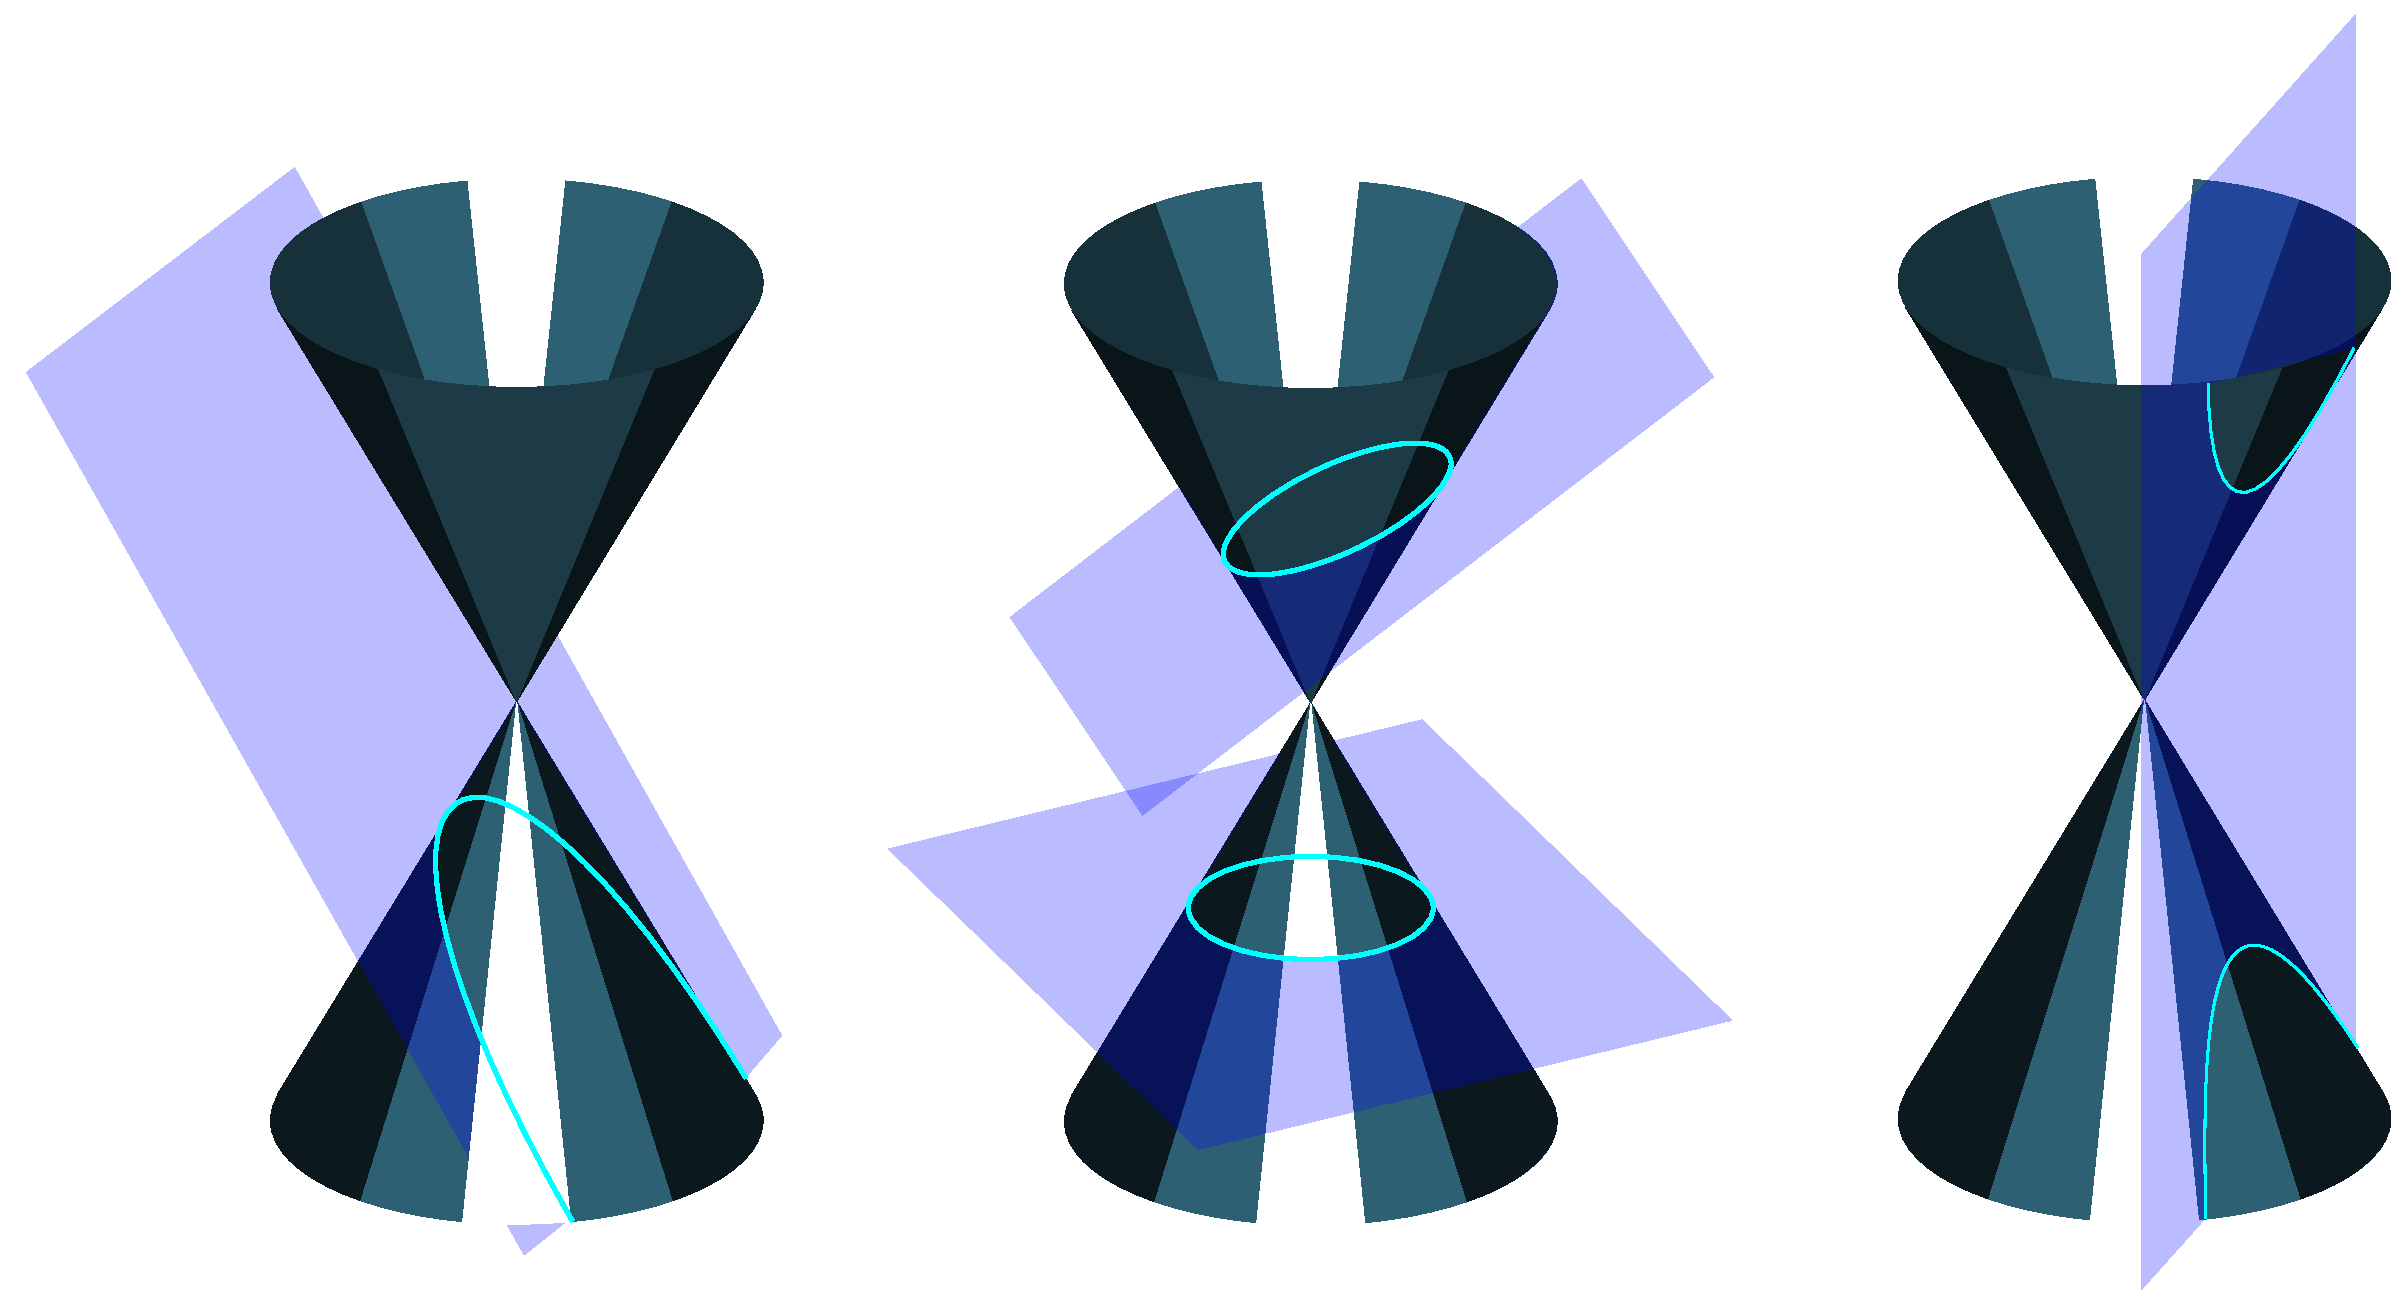
\includegraphics[keepaspectratio,width=10cm]{img/conic_sections.pdf}
		\caption{Die drei Arten von Kegelschnitten, die entstehen, wenn $K$ mit einer Ebene geschnitten wird. \cite{conic}}
	\end{figure}
	
	Eine Ebene im $\RR^3$ wird durch eine Gleichung der Form $ax + by + cz = d$ mit geeigneten Koeffizienten $a,b,c,d \in \RR$ beschrieben, wobei mindestens einer der Koeffizienten $a,b,c \neq 0$ sein muss.
	Ist $c \neq 0$, so folgt $z = \frac{1}{c} (d-ax-by)$.
	Einsetzen in die Kegelgleichung liefert
	\[
		x^2 + y^2 = \frac{1}{c^2} (d-ax-by)^2 = \frac{1}{c^2}(d^2 + a^2x^2 + b^2y^2 + 2abxy - dax - dby),
	\]
	also
	\begin{align*}
		0 &= \enb{\frac{a^2}{c^2}-1}x^2 + \enb{\frac{b^2}{c^2}-1}y^2 + \frac{2ab}{c^2} xy - \frac{2da}{c^2}x - \frac{2db}{c^2}y \\
		\Leftrightarrow \quad 0 &=(a^2-c^2)x^2 + (b^2-c^2)y^2 + 2abxy - 2dax - 2dby.
	\end{align*}
	Durch Wahl geeigneter Parameter bekommt man so alle Typen von Quadriken außer $\emptyset$ oder parallele Geradenpaare bzw. die $y$-Achse als Projektion von $K \cap E$ auf die $x$-$y$-Ebene.
\end{beispiel}

\newpage
